\documentclass[aspectratio=169]{../latex_main/tntbeamer}  % you can pass all options of the beamer class, e.g., 'handout' or 'aspectratio=43'
\usepackage{dsfont}
\usepackage{bm}
\usepackage[english]{babel}
\usepackage[T1]{fontenc}
%\usepackage[utf8]{inputenc}
\usepackage{graphicx}
\graphicspath{ {./figures/} }
\usepackage{algorithm}
\usepackage[ruled,vlined,algo2e,linesnumbered]{algorithm2e}
\usepackage{hyperref}
\usepackage{booktabs}
\usepackage{mathtools}

\usepackage{amsmath,amssymb}

\DeclareMathOperator*{\argmax}{arg\,max}
\DeclareMathOperator*{\argmin}{arg\,min}

\usepackage{amsbsy}
\newcommand{\vect}[1]{\bm{#1}}
%\newcommand{\vect}[1]{\boldsymbol{#1}}

\usepackage{pgfplots}
\pgfplotsset{compat=1.16}
\usepackage{tikz}
\usetikzlibrary{trees} 
\usetikzlibrary{shapes.geometric}
\usetikzlibrary{positioning,shapes,shadows,arrows,calc,mindmap}
\usetikzlibrary{positioning,fadings,through}
\usetikzlibrary{decorations.pathreplacing}
\usetikzlibrary{intersections}
\pgfdeclarelayer{background}
\pgfdeclarelayer{foreground}
\pgfsetlayers{background,main,foreground}
\tikzstyle{activity}=[rectangle, draw=black, rounded corners, text centered, text width=8em]
\tikzstyle{data}=[rectangle, draw=black, text centered, text width=8em]
\tikzstyle{myarrow}=[->, thick, draw=black]

% Define the layers to draw the diagram
\pgfdeclarelayer{background}
\pgfdeclarelayer{foreground}
\pgfsetlayers{background,main,foreground}

% Requires XeLaTeX or LuaLaTeX
%\usepackage{unicode-math}

\usepackage{fontspec}
%\setsansfont{Arial}
\setsansfont{RotisSansSerifStd}[ 
Path=../latex_main/fonts/,
Extension = .otf,
UprightFont = *-Regular,  % or *-Light
BoldFont = *-ExtraBold,  % or *-Bold
ItalicFont = *-Italic
]
\setmonofont{Cascadia Mono}[
Scale=0.8
]

% scale factor adapted; mathrm font added (Benjamin Spitschan @TNT, 2021-06-01)
%\setmathfont[Scale=1.05]{Libertinus Math}
%\setmathrm[Scale=1.05]{Libertinus Math}

% other available math fonts are (not exhaustive)
% Latin Modern Math
% XITS Math
% Libertinus Math
% Asana Math
% Fira Math
% TeX Gyre Pagella Math
% TeX Gyre Bonum Math
% TeX Gyre Schola Math
% TeX Gyre Termes Math

% Literature References
\newcommand{\lit}[2]{\href{#2}{\footnotesize\color{black!60}[#1]}}

%%% Beamer Customization
%----------------------------------------------------------------------
% (Don't) Show sections in frame header. Options: 'sections', 'sections light', empty
\setbeamertemplate{headline}{empty}

% Add header logo for normal frames
\setheaderimage{
	% 
\includegraphics[height=\logoheight]{figures/TNT_darkv4.pdf}
	
\includegraphics[height=\logoheight]{../latex_main/figures/luh_logo_rgb_0_80_155.pdf}
	% 
\includegraphics[height=\logoheight]{figures/logo_tntluh.pdf}
}

% Header logo for title page
\settitleheaderimage{
	% 
\includegraphics[height=\logoheight]{figures/TNT_darkv4.pdf}
	
\includegraphics[height=\logoheight]{../latex_main/figures/luh_logo_rgb_0_80_155.pdf}
	% 
\includegraphics[height=\logoheight]{figures/logo_tntluh.pdf}
}

% Title page: tntdefault 
\setbeamertemplate{title page}[tntdefault]  % or luhstyle
% Add optional title image here
%\addtitlepageimagedefault{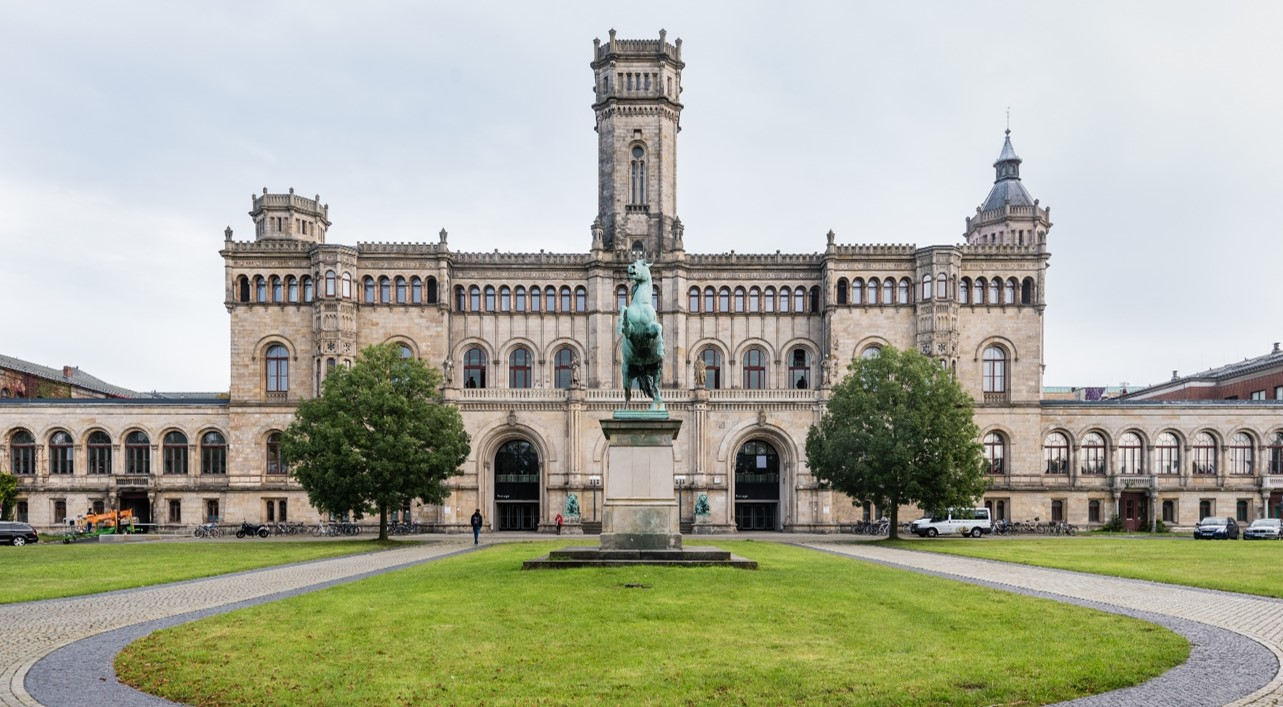
\includegraphics[width=0.65\textwidth]{figures/luh_default_presentation_title_image.jpg}}

% Title page: luhstyle
% \setbeamertemplate{title page}[luhstyle]
% % Add optional title image here
% \addtitlepageimage{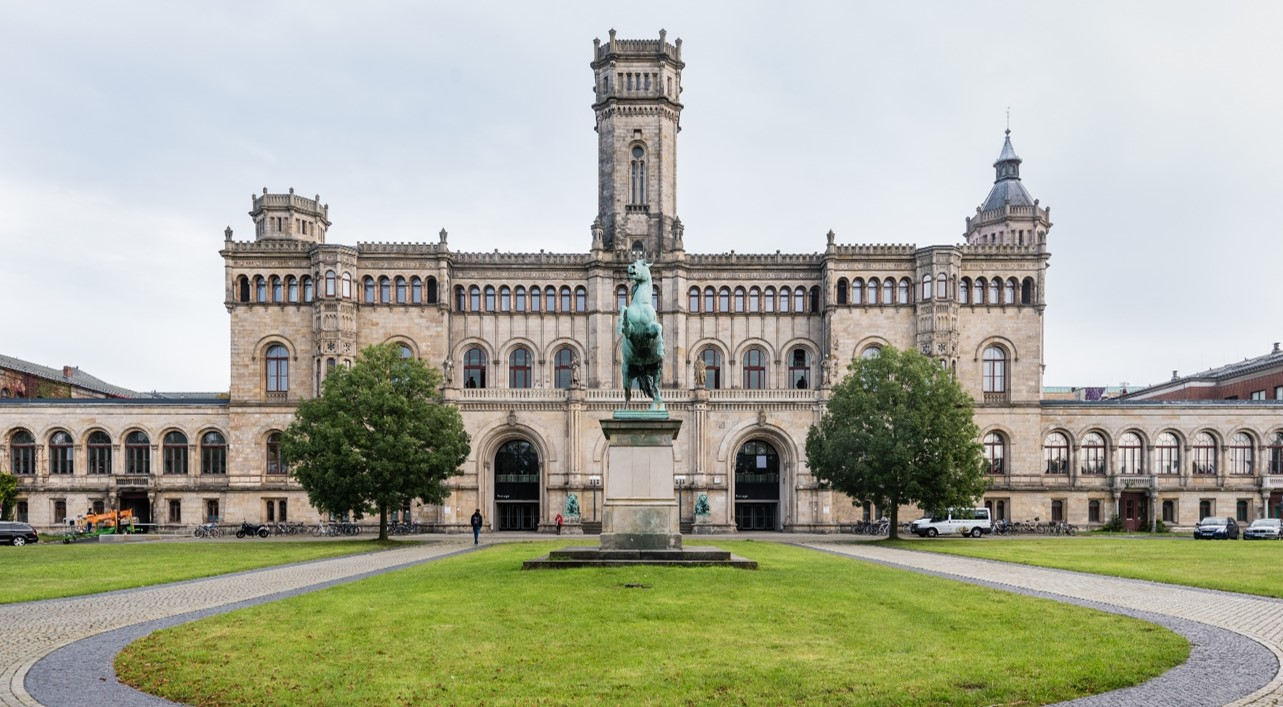
\includegraphics[width=0.75\textwidth]{figures/luh_default_presentation_title_image.jpg}}

\author[Abedjan \& Lindauer]{Ziawasch Abedjan \& Marius Lindauer\\[1em]
	
\includegraphics[height=\logoheight]{../latex_main/figures/luh_logo_rgb_0_80_155.pdf}\qquad
	
\includegraphics[height=\logoheight]{../latex_main/figures/DBIS_Kurzlogo.png}\qquad

\includegraphics[height=\logoheight]{../latex_main/figures/TNT_darkv4}\qquad

\includegraphics[height=\logoheight]{../latex_main/figures/L3S.jpg}	}
\date{Summer Term 2022; \hspace{0.5em} {
\includegraphics[height=1.5em]{../latex_main/figures/Cc-by-nc-sa_icon.svg.png}}; based on \href{https://ds100.org/fa21/}{[DS100]}
}


%%% Custom Packages
%----------------------------------------------------------------------
% Create dummy content
\usepackage{blindtext}

% Adds a frame with the current page layout. Just call \layout inside of a frame.
\usepackage{layout}


%%% Macros
%\renewcommand{\vec}[1]{\mathbf{#1}}
% \usepackage{bm}
%\let\vecb\bm

\title[Regression]{DS: Simple Linear Regression}
\subtitle{Multiple linear regression}

\graphicspath{ {./figure/} }
%\institute{}


\begin{document}
	
	\maketitle
	\begin{frame}{Terminology}
	    There are several equivalent terms in the regression context. You should be aware of them.\\
	    \begin{figure}
	        \centering
	        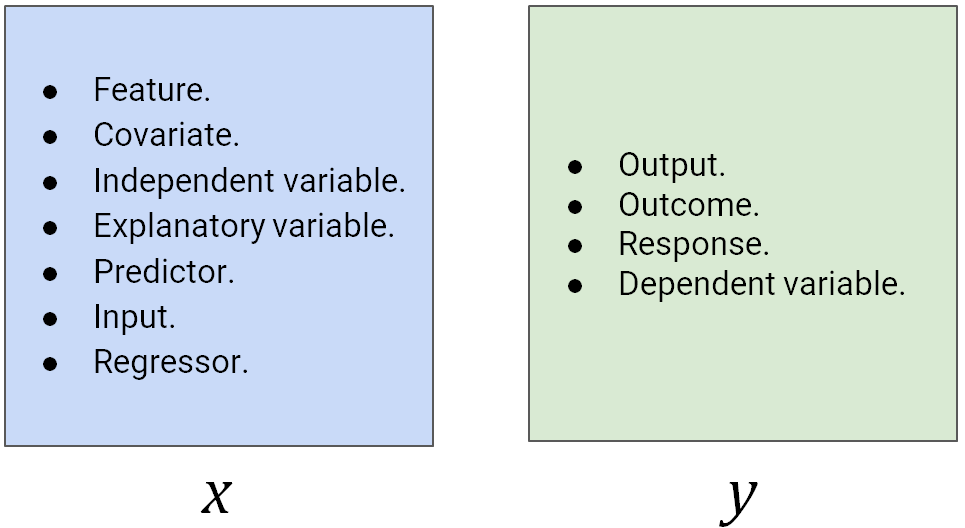
\includegraphics[scale=.42]{Bild9}
	    \end{figure}
        
	\end{frame}
	
	
	
	\begin{frame}{Adding independent variables}
	    
	    \begin{itemize}
	        \item First, some terminology. For our purposes, all of these terms mean the same thing:
    	    \begin{itemize}
    	        \item feature, covariate, independent variable, explanatory variable, predictor, input, regressor.
    	    \end{itemize}
    	    \item In the regression context, each of the above terms has a ``weight'' assigned to it, given by the parameter
    	    \item Weights also called ``coefficients''
    	    \item $\hat{y} = \theta_0 + \theta_1x$:\\
    	    we might say the “weight” associated with the constant/intercept term is $\theta_0$,\\ and the “weight” associated with the $x$ term is $\theta_1$ 
	    \end{itemize}
	    
	\end{frame}
	
	
	\begin{frame}{Adding independent variables}
	    A linear regression model with two features (and thus, three parameters), is of the form
        \begin{equation*}
            \hat{y} = \theta_0 + \theta_1x_1 + \theta_2x_2 
        \end{equation*}
        For example, suppose we want to create a linear regression model that predicts the number of points a player in the NBA averages (PTS). Using just the number of assists (AST) they average might yield a model of the form
        \begin{align*}
            \text{prediction PTS = 3.98 + 2.4} \cdot \text{AST}
        \end{align*}
        If we use both AST and the number of 3PT field goal attempts they make (3PA), we may have
        \begin{align*}
            \text{prediction PTS = 2.163 + 1.64} \cdot \text{AST + 1.26} \cdot 3\text{PA}
        \end{align*}

	\end{frame}
	
	
	\begin{frame}{Visualizing higher-dimension models}
	    In both of the below plots, the blue circles represent the true observations. 
        \begin{itemize}
            \item On the left, the red line represents the model obtained by using only AST.
            \item On the right, since we now have two independent variables, our model is a plane in 3D.
        \end{itemize}
        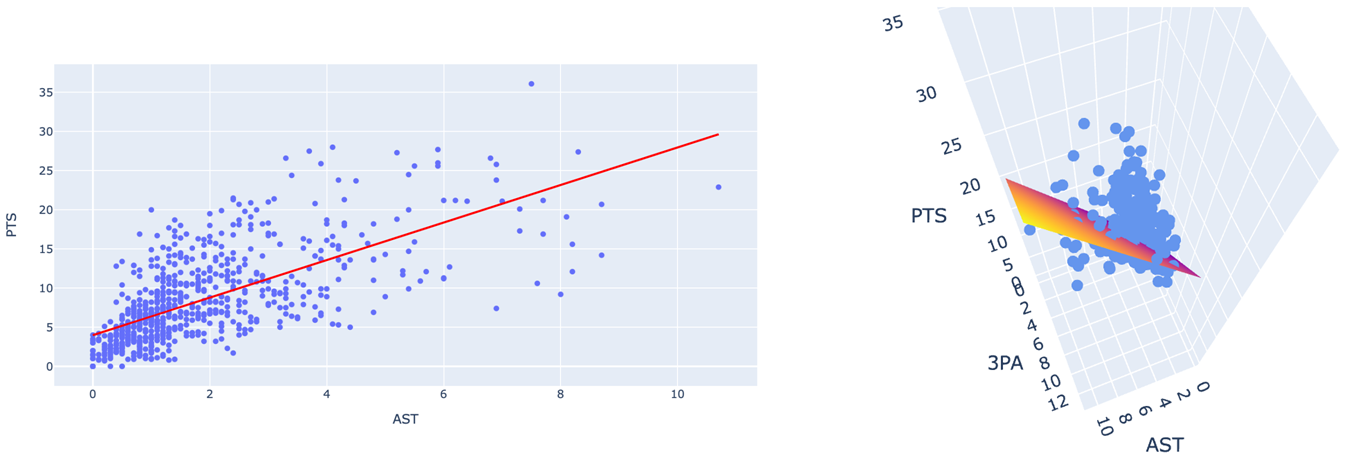
\includegraphics[scale=.4]{Bild10}
	\end{frame}
	
	
	
	\begin{frame}{Multiple linear regression}
	    In general, the multiple linear regression model is of the form
        \begin{equation*}
            \hat{y} = \theta_0 + \theta_1x_1 +  \theta_2x_2 + \theta_3x_3 + ... + \theta_px_p = \theta_0 + \sum_{j=1}^n\theta_jx_j
        \end{equation*}
        
        \begin{itemize}
            \item We say this model has $n$ features, plus an intercept term.
            \item The weight associated with feature $x_j$ is $\theta_j$   .
            \item If we introduce $x_0  = 1$  for each observation, then we can simplify further: $\hat{y} = \sum_{j=0}^n \theta_j x_j$
            \item This is the notation we will use moving forward
            \begin{itemize}
                \item Think about how you can rewrite this in terms of a vector multiplication!
            \end{itemize}
        \end{itemize}
	\end{frame}
	
	
	
	\begin{frame}{Multiple linear regression}
        \begin{align*}
            &\text{model 1: predicted PTS = 3.98 + 2.4}\cdot \text{AST}\\
            &\text{model 2: predicted PTS = 2.163 + 1.64}\cdot \text{AST + 1.26}\cdot \text{3PA}\\
        \end{align*}
        These are different models! In general, $\hat{\theta}_j$ in one model will not be equal to $\hat{\theta_j}$ in another model.
        \begin{itemize}
            \item 2.4 is the slope of the relationship between AST and PTS, when only considering those two variables.
            \begin{itemize}
                \item Parameters [3.98, 2.4] minimize average squared loss for Model 1.
            \end{itemize}
            \item 1.64 is the slope of the relationship between AST and PTS, when also considering 3PA.
            \begin{itemize}
                \item Parameters [2.163, 1.64, 1.26] minimize average squared loss for Model 2.
            \end{itemize}
        \end{itemize}

	\end{frame}
	
	
	
	\begin{frame}{General notation}
        Our models can be expressed as a function         $\hat{y} = f_\theta (x)$             of an input variable, x.\\
        Constant model: $f_\theta (x) = \theta$\\
        Simple linear regression model: $f_\theta (x) = \theta_0 + \theta_1x$\\
        Multiple linear regression model: $f_\theta (x) = \theta_0 + \theta_1x_1 + \theta_2x_2 + ... + \theta_px_p $\\
        \bigskip
        \begin{itemize}
            \item Note: In the latter two models, $\theta$ is a vector, not a scalar! In the last model, $x$ is a vector too. 
            \item We denote the prediction function that uses the optimal choice of parameters for a given loss and model with $f_\hat{\theta}(x)$. For instance, for the SLR  model, $f_\hat{\theta}(x) = \hat{\theta}_0 + \hat{\theta}_1x$                              
            \begin{itemize}
                \item Parameters [2.163, 1.64, 1.26] minimize average squared loss for Model 2.
            \end{itemize}
        \end{itemize}

	\end{frame}
\end{document}